\documentclass[twocolumn]{article}
\usepackage{authblk}
\usepackage{amsmath}
\usepackage{graphicx}
\usepackage{textcomp}
\usepackage{color}
\usepackage{blindtext}
\usepackage{listings}
\usepackage{abstract}
\lstset{language=Matlab}

\begin{document}
\title{LAB ROTATION REPORT \\ }
\date{01.04.2013}
\author[1]{\c{S}eyma BAYRAK\thanks{seyma.bayrak@st.ovgu.de} } 
\affil[1]{\footnotesize  Otto von Guericke University of Magdeburg, Supervisor: Prof. J. Braun}
\maketitle
\newpage

\twocolumn[
\begin{@twocolumnfalse}
\begin{abstract}
My lab rotation in Cognitive Biology Group at Magdeburg University has had two main tasks: experimental and computational tasks. Experimental part aimed to pilot random walk experiment with 3-dimensional rotation, and eliminate a psychometric function of the perception. The stimuli of this task has been prepared by A. Pastukhov, I basically run the stimuli and plot my perception fraction versus life-time of dots on the screen. As expected, when the dots stay longer on the screen, the perception of the observer gets more precise. The core point of this experiment was to find out the lower-limit for the lifetime for the dots, at which the observer starts well-perceiving. The computational part was basically the use of Wilson-Cowan model to express the perception theoretically, which has been preciously expressed experimentally. The Wilson-Cowan model has been analyzed in a detail in the "Computational Task" section. 
\\ 
\end{abstract}
\end{@twocolumnfalse}  ]

 \section{Introduction}
This lab rotation has started at the very beginning with understanding such terms as ``Random-Dot Kinematogram'', ``Psychometric Function'' and ``Hysteresis Loop and Visual System''. This section intends to bring a simple understanding to those key terms, which are crucial in any Psychophsics Lab.
\subsection{Random Dot Kinematogram}
Random-dot kinematogram (RDK) is a special class of visual stimuli for investigating how local motion is integrated into global motion$^{[1]}$. It can be thought as a stimulus of high population of dots moving independently or in a harmony. The harmony is called as ``coherence'', and the independency is referred as ``randomness''. RDK offers only two possible perception to the observer: a coherent perception either exists or not. Let us explain this phenomena by the following example. If the coherence fraction 100 \%, then the observer is expected to ``perceive``, if it is 0 \%, not to ''perceive``.
\begin{center}
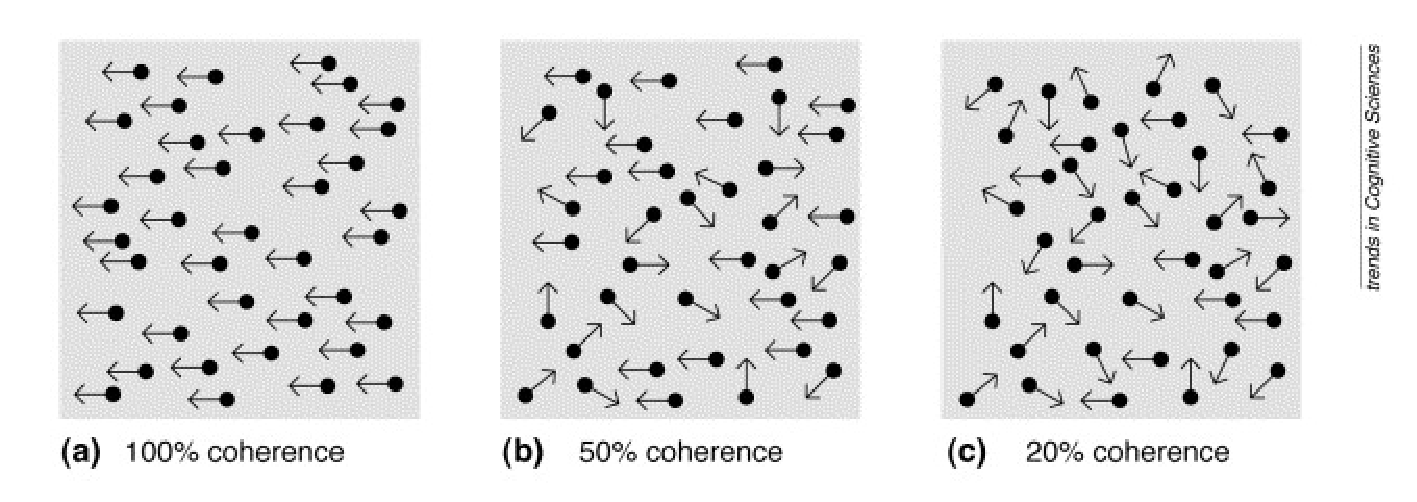
\includegraphics[width=80mm,height=30mm]{RDK.eps} 
   \begin{footnotesize} Figure 1: The coherence level of moving dots in an example stimuli (www.sciencedirect.com).  \end{footnotesize}
\end{center}
\subsection{Psychometric Function}
The Psychometric function is actually a graph rather than a mathematical function. This graph basically reflects the relation between a parameter of the stimulus e.g. coherence level, intensity, lifetime - any property of stimulus, and the perception of the subject e.g. hearing, seeing - a sensation related decision of the subject. Usually the perception of the observer is given as a fraction.
\begin{center}
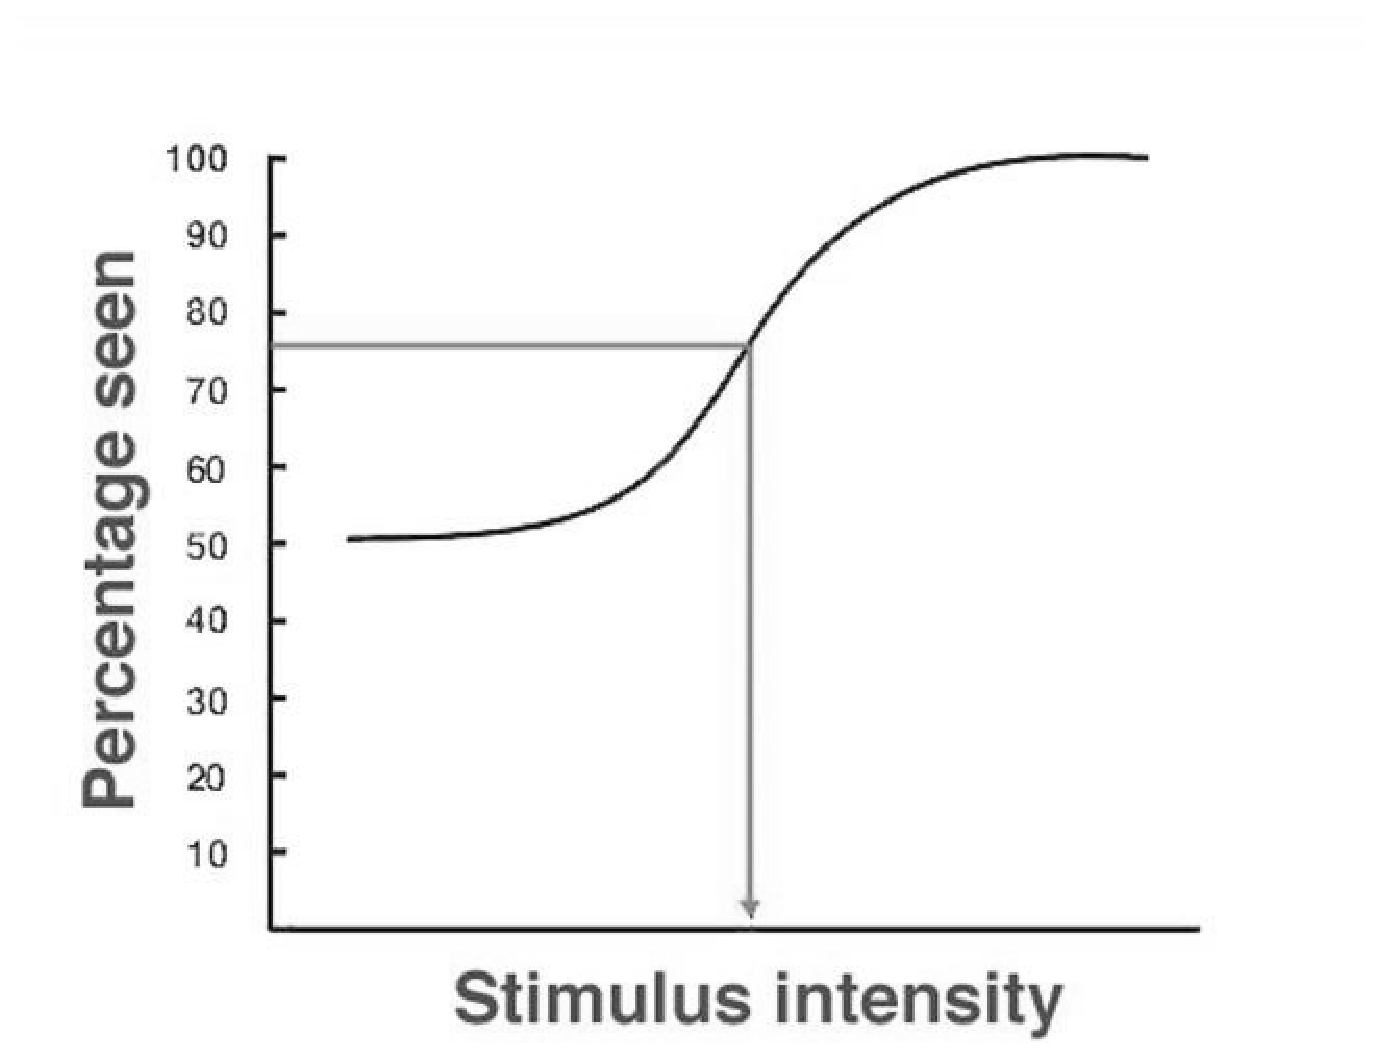
\includegraphics[width=80mm,height=60mm]{psycho.eps} 
   \begin{footnotesize} Figure 2: An example to the psychometric function. As long as the stimuli intensity increases, the better perception of the subject is observed. (webvision.med.utah.edu).  \end{footnotesize}
\end{center}
\subsection{Hysteresis in Motion Binding}
The basic definition of the word hysteresis is the history-dependence of a function. In other words, the behavior of that function depends not only on the parameters of its current state, but also the experience of that function in past. Hysteresis property may appear in the non-linear systems having more than one internal state. 

Now, what is the relation between hysteresis and motion binding? The most simply; the perception of the subject at time $t$ is not only affected by the stimulus at $t$, but also by the previous stimulus that the subject has already seen before time $t$. 
In dynamical system terms, hysteresis implies the existence of range of stimulus strength for which the perceptual representation is bistable in the sense that it offers both a lower activity steady state (associated with a failed percept) and a high activity steady state (associated with a successful percept) $^{[2]}$. This will be further explained by Figure 8. 

\section{Experimental Task}

The purpose of experimental task was to figure out a lower bound for the lifetime of the 3D moving dots to be perceived at first. Once the lifetime of dots was determined, dots having that specific lifetime was used to create another stimulus as seen in Figure 9. The last step was to eliminate a psychometric function indicating fraction of correct percept on y axis and width of this step function shaped stimulus. The first psychometric function derived from the first experiment to define the lifetime is given below. 
\begin{center}
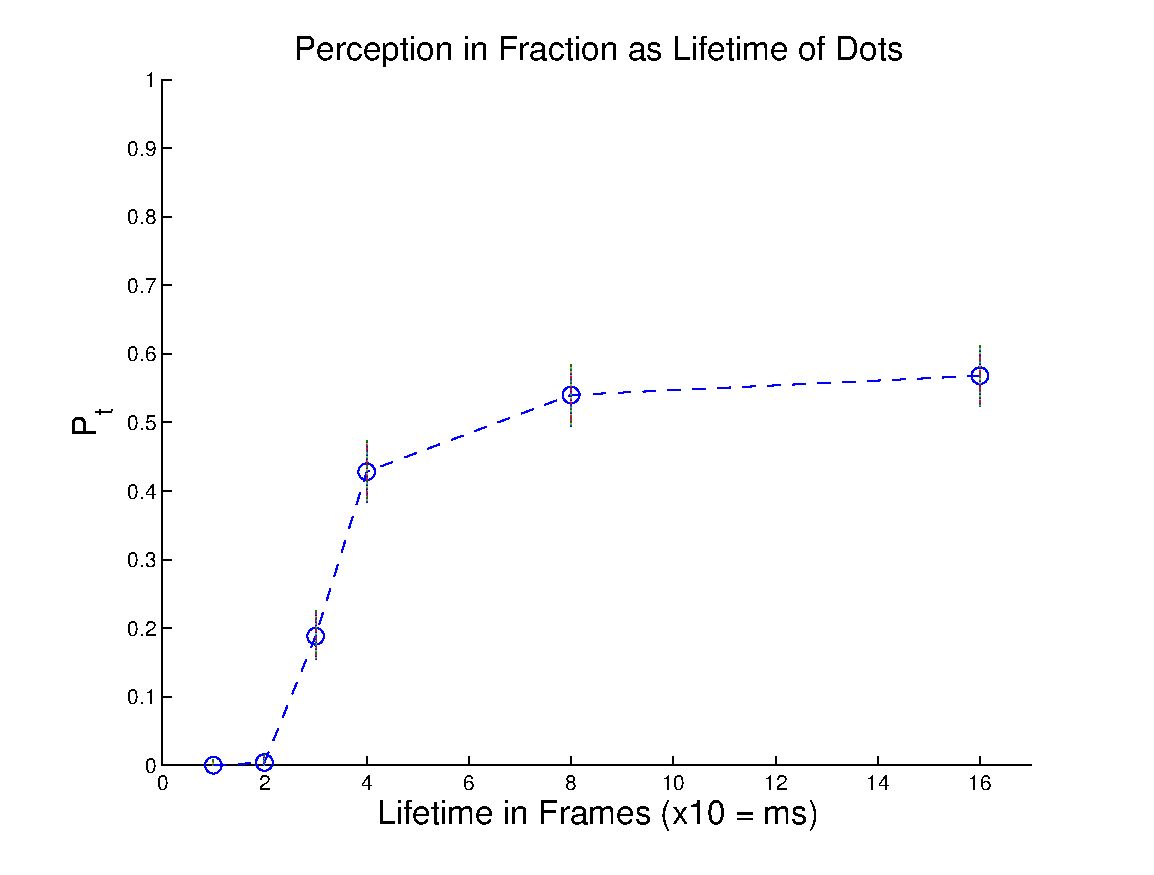
\includegraphics[width=80mm,height=60mm]{p_correct.eps} 
   \begin{footnotesize} Figure 3: Psychometric function to determine the minimum lifetime of dots, it is chosen to be 40 ms. \end{footnotesize}
\end{center}

 \section{Computational Task}
Wilson-Cowan model introduces a solution to the derivative of a time dependent activity $x(t)$ by considering an external input $s(t)$ in addition to Gaussian white noise $\xi(t)$ as the following;

\begin{equation}
 \tau\dot{x}(t)=-x+\Phi(x,s)+\sigma\sqrt{\tau}\xi(t)
\end{equation}
\begin{equation*}
\rightarrow dx(t)=-\frac{x}{\tau}dt+\frac{1}{\tau}\Phi(x,s)dt+\frac{\sigma}{\sqrt{\tau}}n(t)\sqrt{dt} 
\end{equation*}
where $\tau$ is the time constant, $\sigma$ is the amplitude of the Gaussian white noise, and $\Phi(x,s)$ is the \textit{generalized logistic function (GLF)} depending on the input $s(t)$.

\subsection{GLF}
In order to compute the activity $x(t)$ iteratively as Wilson-Cowan model suggests, GLF must be defined properly. The generalized logistic function (GLF) is expressed below, as suggested by Maurizio $^{[2]}$. 

\begin{equation}
 \Phi(x)=(1+e^{-\beta x+\alpha})^{-1/\nu}
\end{equation}

Either equation 1 or 2 are not trivial to fit the computed or expected activity $x(t)$ ideally to the experimental result plots, since they both depend on many parameters such that $\tau$, $\sigma$, $\beta$, $\alpha$ and $\nu$. Those parameters must be chosen well reasonably. My lab rotation has actually started with the analysis of GLF function, how it looks like with different parameters. This subsection reflects the shape of GLF function under change of its parameters.

 
\subsubsection{Inflection Point and $~ \nu$}
Inflection point on a curve is basically defined as the point at which curvature changes sign, or the second derivative of the curve equals to zero. When equation 2 is reduced to the form of $\Phi''(x)=0$, the inflection point's parameters seem to be as in the following:
\begin{equation*}
 x_{inf}=\dfrac{\alpha-ln\nu}{\beta},   \;\;\;\;\;\;        y_{inf}=(1+\nu)^{-1/\nu}
\end{equation*}

Once the $y_{inf}$ is chosen, the $\nu$ parameter can be calculated. A more sophisticated explanation could be more like that, once it is determined when the curvature of GLF changes its sign, then $\nu$ is found out automatically.  

\begin{center}
\includegraphics[width=80mm,height=60mm]{inflection_point.eps} 
   \begin{footnotesize} Figure 4 : The relation between the parameter $\nu$ and the inflection point on y axis. As long as $\nu$ is less than 0, then y is smaller than 1/e, otherwise y is greater than 1/e. Note that the singularity at 0.  \end{footnotesize}
\end{center}

What about the slope just at the inflection point? The slope is found by taking first derivative of GLF given by equation 2. 
\begin{equation*}
\Phi'(x)=y'_{inf}=\beta(1+\nu)^{-1-1/\nu}   
\end{equation*}

\subsubsection{Bisection Point and $\beta$, $\alpha$}
The bisection point divides GLF into two equal parts. In case GLF is restricted as having values between 0 and 1, the bisection point of it is $\Phi(x)=0.5=y_{1/2}$. Equation 2 yields up $x_{1/2}$ as stated below.
\begin{equation*}
 x_{1/2}=\dfrac{\alpha-ln(2^{\nu}-1)}{\beta}
\end{equation*}
Moreover, the slope of GLF function exactly at that bisection point can be expressed by in terms of the parameters. 
\begin{equation*}
 y'_{1/2}=\dfrac{\beta}{2\nu}(1-2^{-v})
\end{equation*}

\subsubsection{Start from Inflection and Plot GLF}
Let us summarize step by step how to eliminate GLF: assign values to inflection points $y_{inf}$, $x_{inf}$ and slope at inflection $y'_{inf}$. Now, the $\nu$ value can be calculated, (e.g. \textit{fsolve} command on MATLAB), $\beta$ can be found through the formula giving $y'_{inf}$ , and $\alpha$ is derived from the formula expresses $x_{inf}$.

\begin{itemize}
\item $\nu=@fsolve((\nu) \;\;\; (1+\nu)^{-1/\nu}-y_{inf})$
\item $\beta=y'_{inf}.(1+\nu)^{1+1/\nu}$
\item $\alpha=\beta.x_{inf}+ln\nu$
\end{itemize}

Let us plot two GLF functions, the assigned parameters are the as the following: for the first GLF (dashed red line); $y_{inf}=0.25$, $x_{inf}=0.5$, $y'_{inf}=1.5$, for the second GLF (solid red line); $y_{inf}=0.75$, $x_{inf}=0.5$, $y'_{inf}=1.5$.  

\begin{center}
\includegraphics[width=80mm,height=60mm]{glf_first.eps} 
   \begin{footnotesize} Figure 5 : The short-solid black lines indicate the slope around inflection points, whereas the blue lines indicate that of bisection points. Note that when $y_{inf}$ is smaller than 1/e, the parameter $\nu$ is smaller than 0.  \end{footnotesize}
\end{center}

\subsubsection{Different $\alpha$ values and GLF }

Now, GLF can be thought more sophisticated as $\Phi(x,s)$ rather than $\Phi(x)$. If $s$ is assumed to be an external input such as a stimuli, and if $\alpha$ is defined as depending on $s$, it is better to express it in a form such that $\Phi(x,s)$. Let us define a linearly changing stimuli  $s=[0 \;\; 0.25\;\; 0.50\;\; 0.75\;\; 1]$ and make $\alpha$ depended on it:
\begin{equation}
 \alpha=\alpha_0+(\alpha_1-\alpha_0).s
\end{equation}
where $\alpha_1$ and $\alpha_0$ are constants. The following GLF function is elliminated. 

\begin{center}
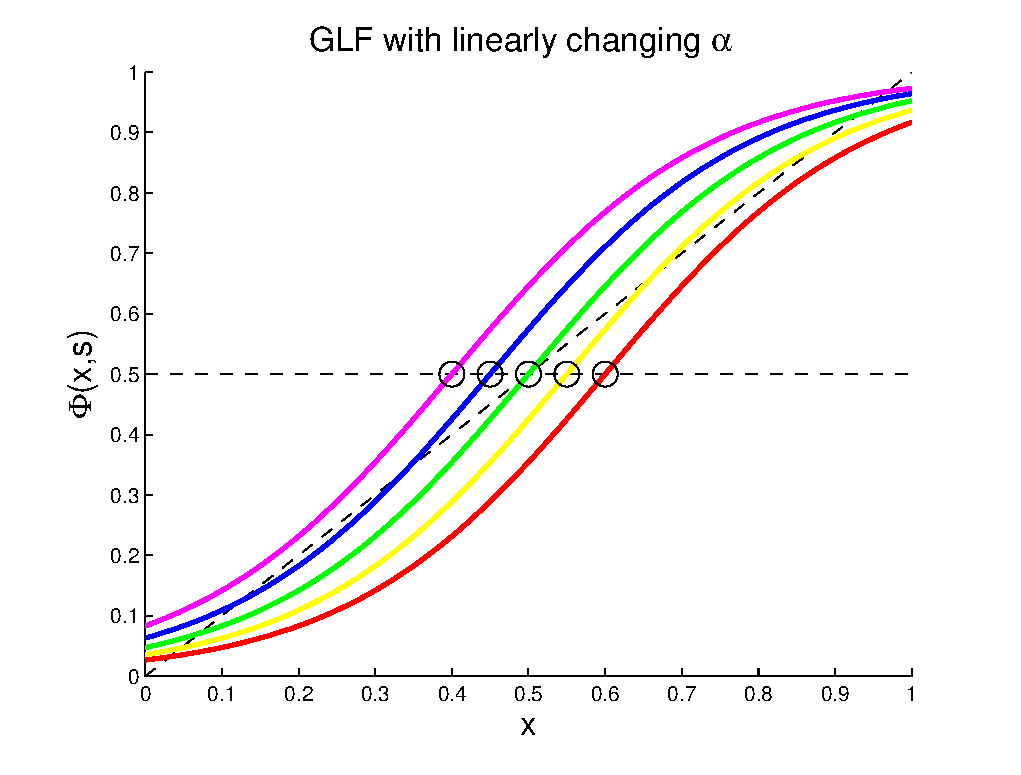
\includegraphics[width=80mm,height=60mm]{linear_alpha.eps} 
   \begin{footnotesize} Figure 6 : As long as $\alpha$ changes, the GLF shifts tothe left around the bisection point. Here, $y_{inf}=0.5$, $y'_{inf}=1.5$, $\alpha$ is given, and the other parameters necessary for GLF are all calculated through the similar steps indicated in section 2.1.3. \end{footnotesize}
\end{center}

\subsubsection{Steady State Points of GLF}
Steady states point are the points where a bifurcation is observed on the GLF function. In other words, steady state points are assumed to be locating on where the sigmoidal-like GLF functions intersects with $x=y$ line. The trick is to assume that $\Phi(x,s) \approx x$ and then let MATLAB find those points with \textit{fsolve} command.
 
\begin{center}
\includegraphics[width=80mm,height=60mm]{steady_state.eps} 
   \begin{footnotesize} Figure 7 : Two GLF with steady state points as indicated as large-black filled up circles. Here, the assigned parameters for the solid line GLF: $y_{inf1}=0.2$, $y'_{inf1}=1.0$, $x_{1/2}=0.55$ and $y_{1/2}=0.5$, for the dashed line GLF:$y_{inf1}=0.2$, $y'_{inf1}=1.0$, $x_{1/2}=0.45$ and $y_{1/2}=0.5$.  \end{footnotesize}
\end{center}

 One single GLF function (with one $\alpha$ parameter) can have maximum three steady state point; those can be categorized as 'high - middle - low steady state points'. Let us now assume that the external input $s$ is changing linearly between 0.1 and 0.9. Therefore the s depended $\alpha$ also changes according to equation 3. The figure below indicates all possible steady state points of many GLF which has different $s$ or in other words different $\alpha$ value each time. 

\begin{center}
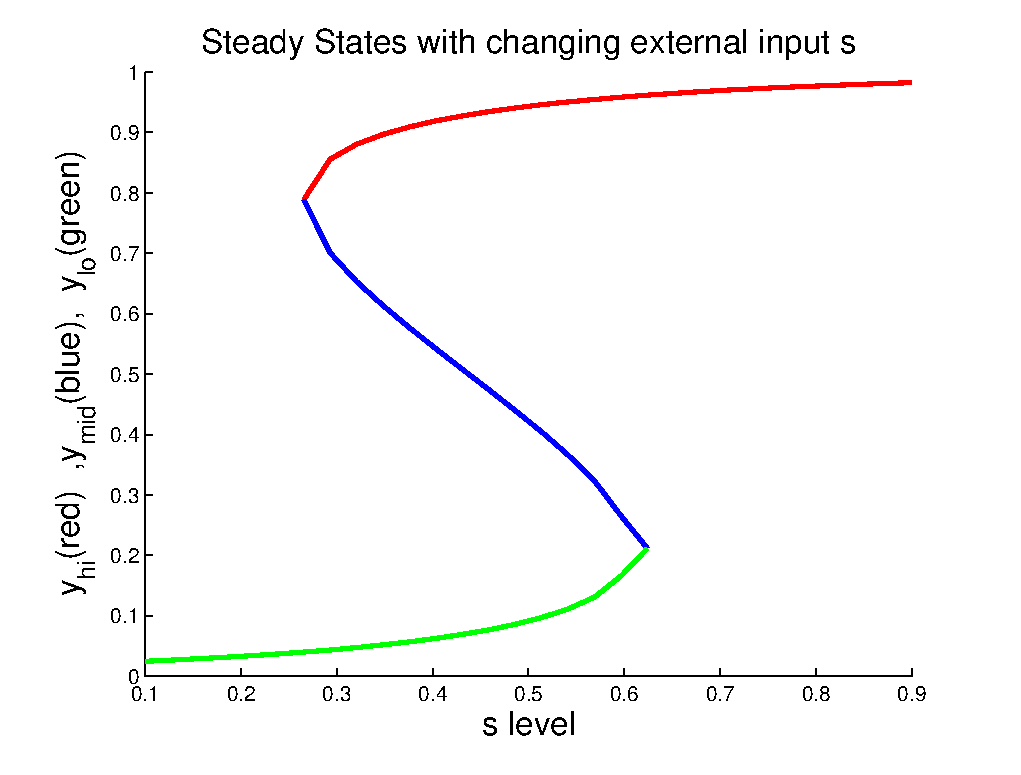
\includegraphics[width=80mm,height=60mm]{s_vs_steadystate.eps} 
   \begin{footnotesize} Figure 8 : Steady state points of different GLF functions corresponding to given $s$ values on x axis. Note that at each s value, there could be maximum three steady state points which could be in high - middle - low transition areas. The fact that "at one stimulus strength, the activity could be around failure area or success area" is related to hysteresis property of visual perception.  \end{footnotesize}
\end{center}


\subsection{Wilson Cowan Model with Step Input}
After analyzing GLF, it is yet simpler to determine the activity $x(t)$ with Wilson-Cowan model. However, GLF is defined as depending on an external parameter called $s$. In fact, this parameter represents the ``coherence'' of the rotating dots in my experiment, so it is an input related to the stimulus. We would like to have very randomly moving dots with 0 coherence during the beginning of stimuli time, then increase coherence up to 100 \% and then reduce it back to an intermediate level around 40 \%. The corresponding $s$ graph is shown below. 

 \begin{center}
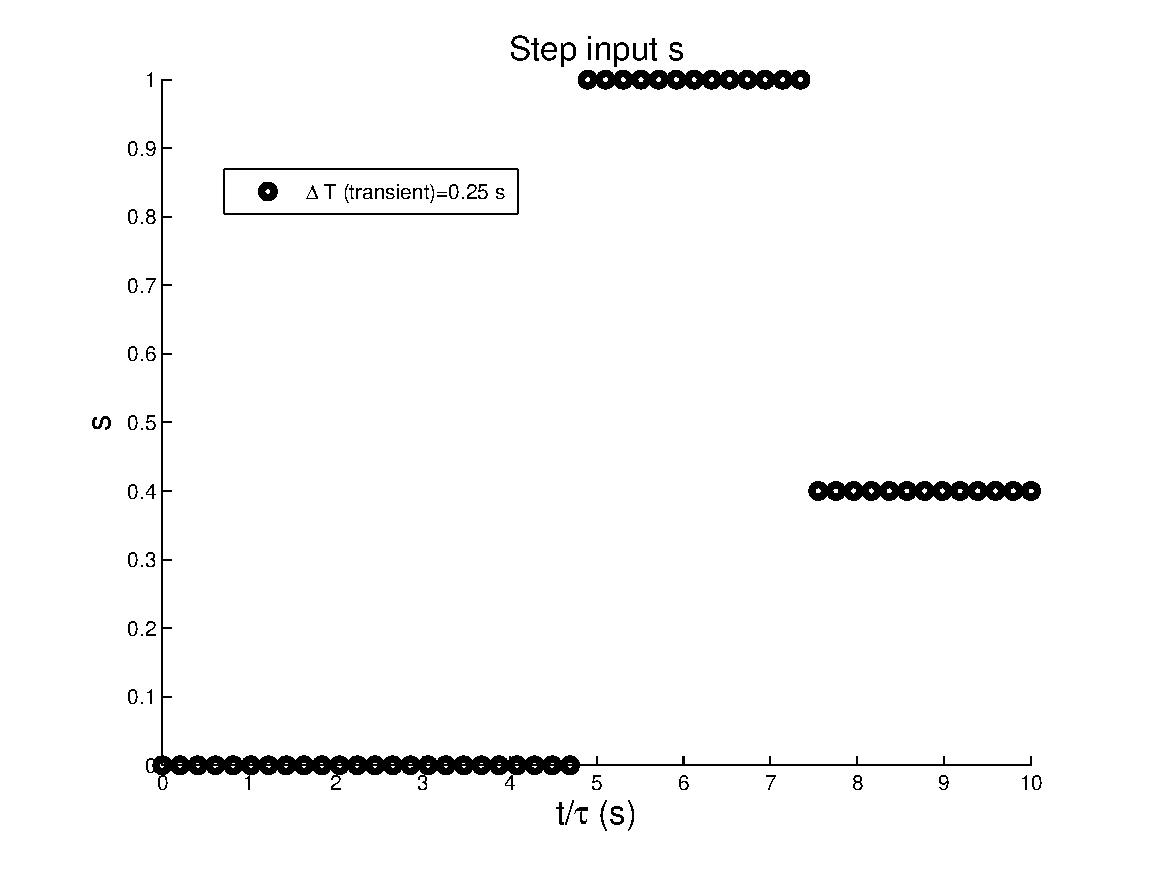
\includegraphics[width=80mm,height=60mm]{step_s.eps} 
   \begin{footnotesize} Figure 9 : A step input level changing in time (divided by time constant on the x axis).  Transient time corresponds to width of maximum coherence in terms of duration. \end{footnotesize}
\end{center}

The well-defined parameters are now inserted into GLF, inclusively the parameter $\alpha$ with the dependence of the step input just shown above. The activity $x(t)$ is calculated by the numerical integration of Equation 1 as Wilson-Cowan model suggested previously. The initial point of the activity $x_0$ is chosen to be 0, this corresponds to "no perception at the beginning" in my experiment.

 \begin{center}
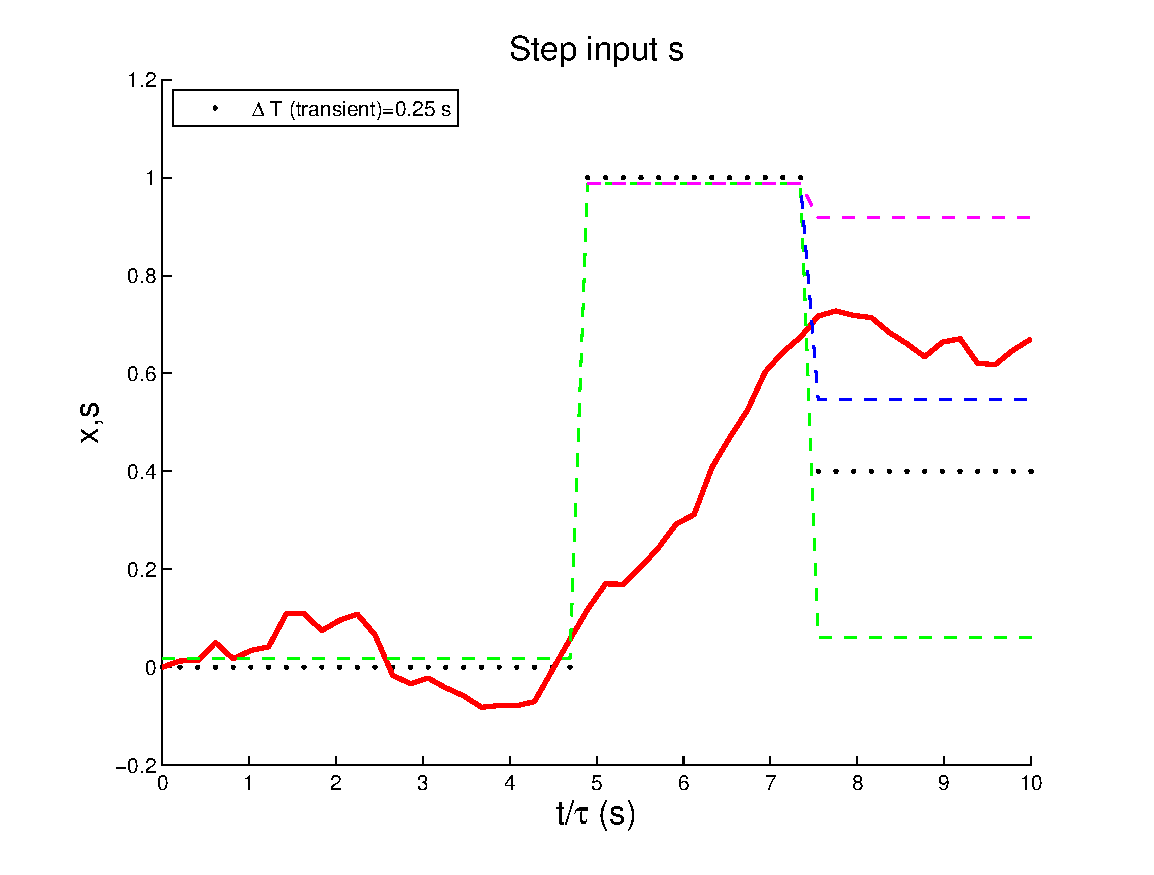
\includegraphics[width=80mm,height=60mm]{my_WC.eps} 
   \begin{footnotesize} Figure 10 : The activity $x$ is reflected as the red line above, black dots represent the step input $s$, and dashed lines stand for the steady state points of GLF for each $s$ value, green for the low steady state points, blue for intermediate transition levels, and magenta for high steady state points.  \end{footnotesize}
\end{center}

\subsection{Activity Probability of $s$ with Different Transient Values}
The whole concern is actually to figure out where the activity $x(t)$ ends up. The activity itself is the theoretical model of the perception of the "observer". The initial value $x_0$ is already chosen to be 0, but the interested value is what $x(t)$ equals to after the total time duration of the model step stimuli. When the last value of $x(t)$ is greater than 0.5, it is assumed that the activity is successful, otherwise failed. To explain it more understandable, let us use Figure 7, there the activity (red curve) ends up somewhere around greater than 0.5, so it is a successful or correct activity.

Since $x(t)$ depends on a Gaussian white noise meaning a series of randomness, the correctness of activity needs to be calculated by a  statistical approach. In my program, I run the program 200 times for each step input coherence $s$ and then got a fraction of successful results of activity overall 200 trials as the following:
\begin{equation}
 P_{correct}=\dfrac{number \;\;\;of\;\;\;correct\;\;\;trials}{number\;\;\;of\;\;\;total\;\;\;trials}
\end{equation}

The last step of my theoretical analysis is to create $s$ with different transient durations. The 100 \% coherence level duration is changed linearly between 0.1 and 0.9 seconds. Then, Wilson-Cowan model is applied to find out the $x$, and $P_{correct}$ is eliminated.

 \begin{center}
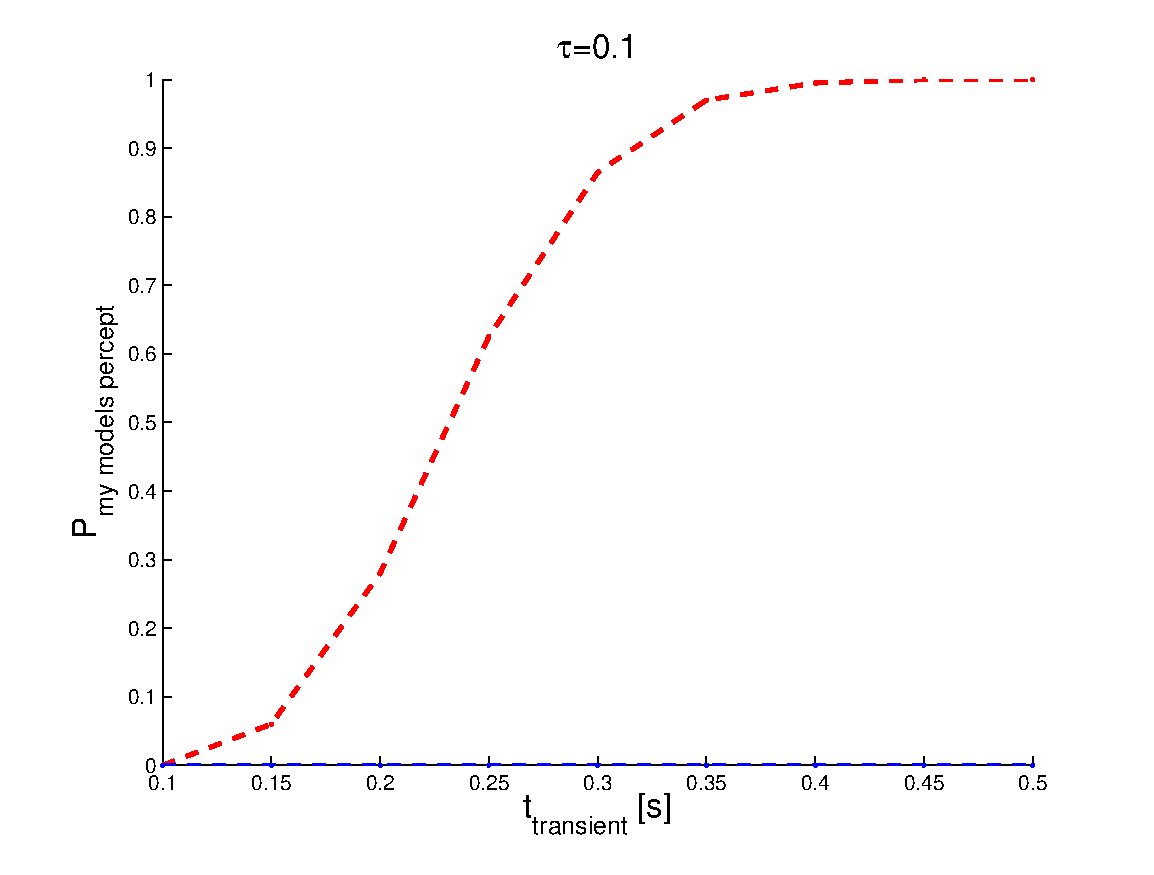
\includegraphics[width=80mm,height=60mm]{my_P_correct.eps} 
   \begin{footnotesize} Figure 11 : The red-dashed line represents the probability of correct activities corresponding to transient durations. The blue-dashed line is the same procedure repeated for the $s$ having no transient duration, it is assumed to be a "baseline".  \end{footnotesize}
\end{center}

\section{References}

[1] http://www.psykinematix.com/documentation
\newline
\newline
[2]``Hysteresis in Motion Binding'', Achim, Guillermo, Mauruzio, Paolo, Sasha. 19 Feb. 2013



\end{document}
